\chapter{Architektur}

Die App sollte mit dem JavaScript-Framework react-native programmiert werden. Dieses Framework wird eingesetzt, wenn die App sowohl auf mobilen IOS-, als auch Android-Geräten funktionieren soll. Auf diese Art wird Code geschrieben werden, welcher für beide Plattformen verwendet werden kann \cite{whyReactNative}. Als Programmiersprache wird TypeScript eingesetzt. TypeScript ist wie JavaScript, nur mit Typensicherheit. So können keine Verwirrungen bezüglich des Typs einer Variable aufkommen \cite{whyTypeScript}. Zusammen mit TypeScript und dem Framework react-native wird zusätzlich noch Expo genutzt. Expo ist ein Framework, welches Werkzeuge zur Unterstützung der Entwicklung einer react-native-App bietet \cite{whyExpo}. 

\section{Mockups und Komponenten}
Um die Anforderungen nicht völlig durcheinander in Quell-Code zu ,,pressen'', werden vorher Prototypen entworfen, welche das Design der App darstellen sollen. Dies schafft Struktur und ermöglicht es, systematisch vorzugehen. Ziel der Mockups ist es, ein Design zu schaffen, welches möglichst einfach und verständlich alle relevanten Informationen auf einen Blick zeigt und es dem Nutzer ermöglicht, sich ebenfalls weitere Details anzeigen zu lassen, wenn dies gewünscht ist. Anhand dieser Mockups gelingt es nun, Komponenten herauszuarbeiten, welche anschließend in Quell-Code umgewandelt werden sollen.

Da die Implementierung mit react-native erfolgt und statt Klassen Komponenten für die Benutzeroberfläche verwendet werden, werden auch die Mockups in Komponenten aufgeteilt. Die Komponente, welche alle anderen beinhalten soll, ist die ,App'. Hier findet sich auch ein Button oben rechts, der in \autoref{fig:mockupApp}(a) zu sehen ist. Eine weitere Komponente bildet die Karte, welche sich über den größten Teil des Bildschirms erstreckt. Wird auf einen Marker geklickt, der eine Parkmöglichkeit anzeigt, so öffnet sich die Komponente der Beschreibung. Diese ist beispielsweise in \autoref{fig:mockupBeschreibung}(b) zu sehen. Hier sollen Kacheln angezeigt werden, welche die einzelnen Informationen liefern. Außerdem soll hier auch der Button angezeigt werden, welcher die Navigation startet. 

\begin{figure}[h!]
	\centering
	\subfloat[\centering Dieser Entwurf zeigt die Komponente ,App' mit dem einem Button oben rechts in der Ecke. Außerdem befindet sich hier auch die Komponente mit der Karte.]{{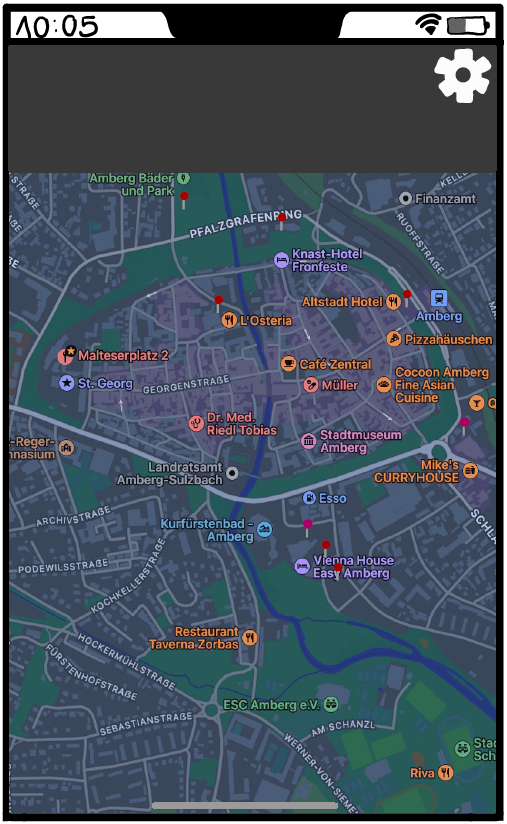
\includegraphics[width=0.45\linewidth]{mockup_app.png}}}
	\qquad
	\subfloat[\centering Zusätzlich zur Karten-Kompnente in der ,App' ist hier auch noch die Komponente der Beschreibung zu sehen, welche sich beim Klick auf eine Parkmöglichkeit in der Karte öffnen soll. Die Kacheln zeigen die relevanten Informationen an.]{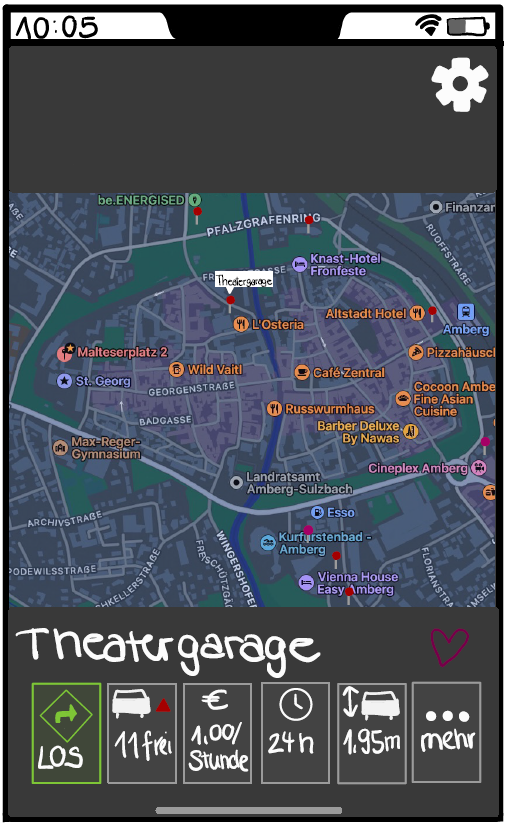
\includegraphics[width=0.45\linewidth]{mockup_beschreibung.png}}
	\caption[Diese beiden Entwürfe zeigen jeweils die ,App'-Komponente und die darin befindliche Karten-Komponente. In der rechten Abbildung öffnet sich zusätzlich die Beschreibung-Komponente, welche die Karte verkleinert.]{Diese beiden Entwürfe zeigen jeweils die ,App'-Komponente und die darin befindliche Karten-Komponente. In der rechten Abbildung öffnet sich zusätzlich die Beschreibung-Komponente, welche die Karte verkleinert. (Quelle: Eigens gezeichnete Mockups)}
	\label{fig:mockupApp}
	\label{fig:mockupBeschreibung}
\end{figure}

Wird auf das Zahnrad in \autoref{fig:mockupApp}(a) in der Komponente ,App' geklickt, so soll sich eine Komponente mit den Einstellungen, wie in \autoref{fig:mockupSettings}(a) zu sehen, öffnen, in welcher der Ton an- und ausgeschaltet werden kann oder auch die Parkmöglichkeiten als Liste angezeigt werden können. Um die Parkmöglichkeiten als Liste zu sehen, wird eine weitere Komponente benötigt, wie sie in \autoref{fig:mockupParkingList}(b) erkennbar ist. Die Elemente der Liste werden mit den Favoriten zuerst und dann nach dem Alphabet sortiert. 

\begin{figure}[h!]
	\centering
	\subfloat[\centering Die Komponente, welche das Einstellungsmenü beinhaltet. Ein Klick auf den Ton schaltet diesen entweder ein oder aus. Die Kachel darunter zeigt bei einem Klick die Parkmöglichkeiten als Liste an.]{{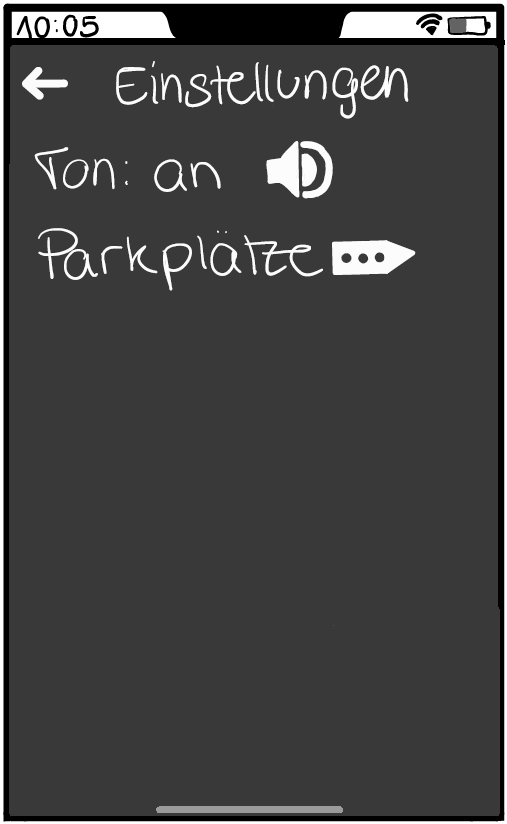
\includegraphics[width=0.45\linewidth]{mockup_settings.png}}}
	\qquad
	\subfloat[\centering Hier befindet sich die Liste der Parkmöglichkeiten, welche alphabetisch sortiert ist. Die Favoriten finden sich hier ganz oben.]{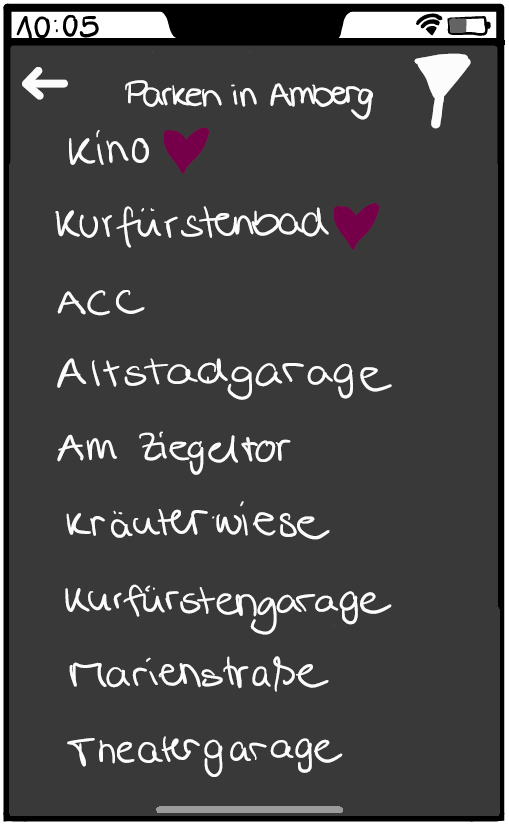
\includegraphics[width=0.45\linewidth]{mockup_parkinglist.png}}
	\caption[Auf den Entwürfen ist links das Einstellungsmenü zu sehen. Wird auf ,Parkplätze' oder in der Beschreibung-Komponente auf ,mehr' geklickt, so wird zur Ansicht der Details einer Parkmöglichkeit, was auf der rechten Seite zu sehen ist, navigiert.]{Auf den Entwürfen ist links das Einstellungsmenü zu sehen. Wird auf ,Parkplätze' oder in der Beschreibung-Komponente auf ,mehr' geklickt, so wird zur Ansicht der Details einer Parkmöglichkeit, was auf der rechten Seite zu sehen ist, navigiert. (Quelle: Eigens gezeichnete Mockups)}
\label{fig:mockupSettings}
\label{fig:mockupParkingList}
\end{figure}
\newpage
Wird in der Liste auf eine Parkmöglichkeit oder in der Beschreibung einer einzelnen auf die Kachel mit der Beschriftung "mehr" geklickt, öffnet sich eine Detailansicht, welche alle vorhandenen Informationen des Parkhauses anzeigt. Zu sehen ist dies in \autoref{fig:mockupParkingDetails} Diese Übersicht bildet die letzte Komponente. 

\begin{figure}[h!]
	\centering
	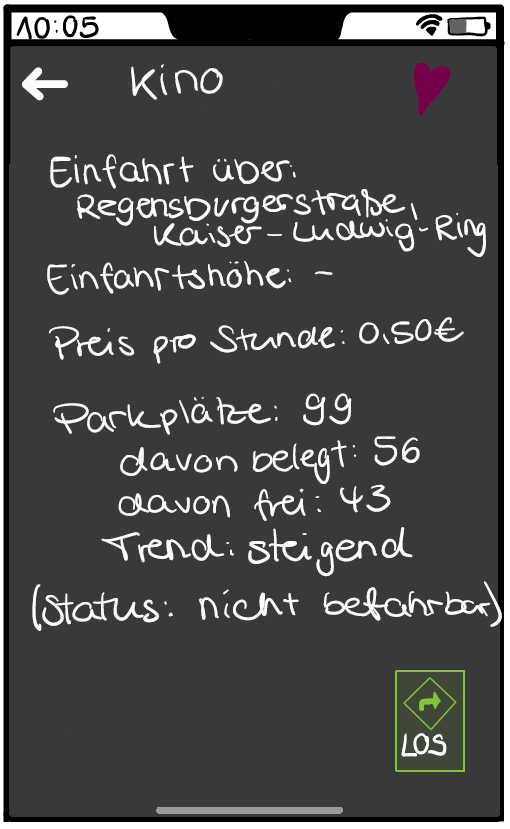
\includegraphics[width=0.45\linewidth]{mockup_parkingdetais.png}
	\caption[Diese Komponente bildet die Detailsansicht der jeweiligen Parkmöglichkeit. Zu erreichen ist diese über die Beschreibung- oder die Einstellung-Komponente.]
	{Diese Komponente bildet die Detailsansicht der jeweiligen Parkmöglichkeit. Zu erreichen ist diese über die Beschreibung- oder die Einstellung-Komponente. (Quelle: Eigens erstellte Übersicht.)}
	\label{fig:mockupParkingDetails}
\end{figure}
\newpage
In Summe sind also zunächst fünf Komponenten geplant, welche in der Komponente ,App' zu finden sind. Ob dies tatsächlich so umsetzbar ist, wird sich in der Implementierung zeigen.

\section{Datenbank}
Um die Daten nun auch sauber vom Code zu trennen, müssen Datenbanktabellen angelegt werden. Die erste Tabelle ,parkingarea' wird mit den Daten der Parkmöglichkeiten gefüllt. Hierzu bekommt jedes der neun Parkmöglichkeiten eine ID zur Identifikation. Weitere Spalten in der Tabelle beinhalten:
\begin{description}
	\item \textbf{Name} \\ Der Name des Parkhauses oder Parkplatzes.
	\item \textbf{Adresse} \\ Die Straße oder mehrere Straßen, über die die Parkmöglichkeit angefahren werden kann.
	\newpage
	\item \textbf{Öffnungszeiten} \\ Wie lange die jeweilige Parkmöglichkeit geöffnet hat.
	\item \textbf{Preis pro Stunde} \\ Wie viel pro Stunde bezahlt werden muss, um sein Fahrzeug zu parken.
	\item \textbf{Einfahrtshöhe} \\ Wie hoch das Fahrzeug maximal sein darf, um in das Parkhaus zu fahren. Im vorliegenden Fall gibt es auch Parkplätze ohne maximale Einfahrtshöhe.
	\item \textbf{Favorit} \\ Dieser Wert gibt an, ob es sich um eine favorisiertes Parkmöglichkeit handelt oder nicht. In dem Fall gibt der Wert 1 eine favorisierte Parkmöglichkeit an, wohingegen 0 anzeigt, dass eine Parkmöglichkeit nicht favorisiert ist.
	\item \textbf{Latitude} \\ Latitude ist die geographische Breite oder auch der Breitengrad. In Zusammenspiel mit dem Längengrad ergibt sich die exakte Position der Parkmöglichkeit auf der Erde.
	\item \textbf{Longitude} \\ Die geographische Länge oder auch Längengrad.
\end{description}
In \autoref{fig:parkingarea} sind alle Spalten der Tabelle ,parkingarea' mit ihren zugehörigen Datentypen zu erkennen.

\begin{figure}[h]
	\centering
	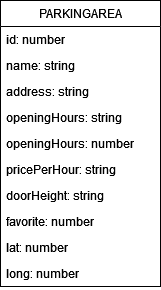
\includegraphics[width=0.2\linewidth]{table_parkingarea.png}
	\caption[Die Spalten und ihre Datentypen der Datenbanktabelle ,parkingarea'. Hier werden in \autoref{implementierung} alle Parkmöglichkeiten eingetragen.]
	{Die Spalten und ihre Datentypen der Datenbanktabelle ,parkingarea'. Hier werden in \autoref{implementierung} alle Parkmöglichkeiten eingetragen. (Quelle: Eigens erstellte Übersicht.)}
	\label{fig:parkingarea}
\end{figure}

Die zweite Datenbanktabelle erhielt den Namen ,parkingareadetails' und sollte mit den Daten der API gefüllt werden. Neben einer einzigartigen ID finden sich hier folgende Spalten: 
\begin{description}
	\item \textbf{ID des jeweiligen Parkhauses} \\ Um die Details der Parkmöglichkeiten denen der anderen Tabelle zuordnen zu können, wird zu jedem Datensatz die ID der Parkmöglichkeit gespeichert, zu der die Informationen gehören.
	\item \textbf{Anzahl der Parkplätze} \\ Die Anzahl der Gesamtheit aller Parkplätze der jeweiligen Parkmöglichkeit, unabhängig davon, ob diese belegt oder frei sind.
	\item \textbf{Anzahl belegter Parkplätze} \\ Die Anzahl der Parkplätze, die aktuell belegt sind.
	\item \textbf{Anzahl freier Parkplätze} \\ Die Anzahl der Parkplätze, auf denen noch geparkt werden kann.
	\item \textbf{Trend} \\ Der Trend gibt an, ob die Anzahl belegter Parkplätze steigt, sinkt oder gleich bleibt. Wenn beispielsweise viele Menschen auf einmal in die Parkmöglichkeit einfahren, so steigt der Trend. Der Trend kann die Werte 0 für ,gleichbleibend', 1 für ,steigend' oder -1 für ,fallend' annehmen.
	\item \textbf{Status} \\ Der Status, in welchem sich die Parkmöglichkeit befindet. Hierfür wird zwischen ,OK', ,Ersatzwerte', ,Manuell' oder ,Störung' unterschieden.
	\item \textbf{Geschlossen} \\ Dieser Wert zeigt an, ob die Parkmöglichkeit aktuell geöffnet oder geschlossen hat. Bei 0 ist die Parkmöglichkeit offen, bei 1 geschlossen.
	\item \textbf{Datum und Uhrzeit der Daten} \\ Um die aktuellsten Daten zu verwenden, müssen Datum und Uhrzeit, zu welcher die Daten erstellt sind, gespeichert werden.
\end{description}
In \autoref{fig:parkingareadetails} sind nochmals alle Spaltenbezeichnungen und die dazugehörigen Datentypen aufgelistet.

\begin{figure}[h]
	\centering
	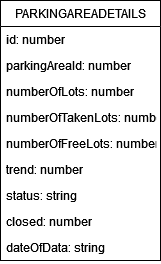
\includegraphics[width=0.2\linewidth]{table_parkingareadetails.png}
	\caption[Um die Daten der API verwenden zu können, wird eine Tabelle ,parkingareadetails' erstellt. Zu sehen sind hier die Spaltenbezeichnungen und die dazugehörigen Datentypen.]
	{Um die Daten der API verwenden zu können, wird eine Tabelle ,parkingareadetails' erstellt. Zu sehen sind hier die Spaltenbezeichnungen und die dazugehörigen Datentypen. (Quelle: Eigens erstellte Übersicht.)}
	\label{fig:parkingareadetails}
\end{figure}